% ============================================================
%  Information Theory --- Module 3 --- ALL DIAGRAMS (merged)
%  Compile with pdfLaTeX.  Each diagram starts on its own page.
%  Auto-merged from Information_Theory_Module3_Solutions.md
% ============================================================
\documentclass[11pt]{article}
\usepackage[a4paper,margin=1.5cm]{geometry}
\usepackage{amsmath}
\usepackage{tikz}
\usetikzlibrary{automata,positioning,arrows.meta,trees,calc}
\usepackage{forest}
\usepackage{pgfplots}
\pgfplotsset{compat=1.18}
\setlength{\parindent}{0pt}
\title{\textbf{Information Theory --- Module 3}\\[2pt] All Diagrams (TikZ / forest / pgfplots)}
\author{}
\date{}
\begin{document}
\maketitle

% ---------- Q6 : diagram 1 ----------
\clearpage
\section*{Q6 --- diagram 1}
\begin{center}
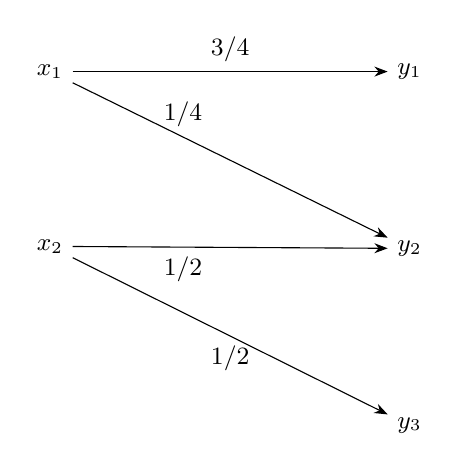
\begin{tikzpicture}[>=Stealth,node distance=1.8cm and 4cm,
   every node/.style={font=\small}]
  \node (x1) {$x_1$};
  \node (x2) [below=of x1] {$x_2$};
  \node (y1) [right=of x1] {$y_1$};
  \node (y2) [below=of y1] {$y_2$};
  \node (y3) [below=of y2] {$y_3$};
  \draw[->] (x1) -- node[above]{$3/4$} (y1);
  \draw[->] (x1) -- node[pos=.35,above]{$1/4$} (y2);
  \draw[->] (x2) -- node[pos=.35,below]{$1/2$} (y2);
  \draw[->] (x2) -- node[below]{$1/2$} (y3);
\end{tikzpicture}
\end{center}

% ---------- Q7 : diagram 2 ----------
\clearpage
\section*{Q7 --- diagram 2}
\begin{center}
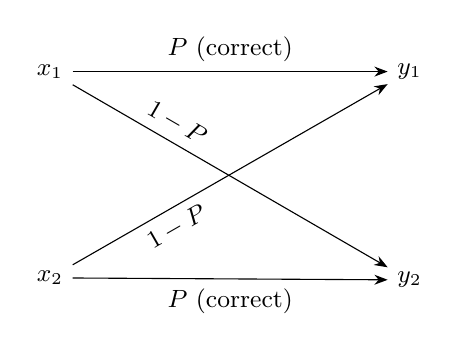
\begin{tikzpicture}[>=Stealth,node distance=2.2cm and 4cm,
   every node/.style={font=\small}]
  \node (x1) {$x_1$};
  \node (x2) [below=of x1] {$x_2$};
  \node (y1) [right=of x1] {$y_1$};
  \node (y2) [below=of y1] {$y_2$};
  \draw[->] (x1) -- node[above]{$P$ (correct)} (y1);
  \draw[->] (x1) -- node[pos=.3,above,sloped]{$1-P$} (y2);
  \draw[->] (x2) -- node[pos=.3,below,sloped]{$1-P$} (y1);
  \draw[->] (x2) -- node[below]{$P$ (correct)} (y2);
\end{tikzpicture}
\end{center}

% ---------- Q8 : diagram 3 ----------
\clearpage
\section*{Q8 --- diagram 3}
\begin{center}
\begin{tikzpicture}[>=Stealth,node distance=2.4cm and 4.5cm,
   every node/.style={font=\small}]
  \node (x1) {$x_1\ (0)$};
  \node (x2) [below=of x1] {$x_2\ (1)$};
  \node (y1) [right=of x1] {$y_1\ (0)$};
  \node (ye) [below=of y1] {$Y$ (erasure)};
  \node (y2) [below=of ye] {$y_2\ (1)$};
  \draw[->] (x1) -- node[above]{$\bar P=1-P$} (y1);
  \draw[->] (x1) -- node[pos=.4,above,sloped]{$P$} (ye);
  \draw[->] (x2) -- node[pos=.4,below,sloped]{$P$} (ye);
  \draw[->] (x2) -- node[below]{$\bar P=1-P$} (y2);
\end{tikzpicture}
\end{center}

% ---------- Q9 : diagram 4 ----------
\clearpage
\section*{Q9 --- diagram 4}
\begin{center}
\begin{tikzpicture}[>=Stealth,node distance=1.4cm and 4.5cm,
   every node/.style={font=\small}]
  \node (x0) {$0$};
  \node (x1) [below=of x0] {$1$};
  \node (x2) [below=of x1] {$2$};
  \node (x3) [below=of x2] {$3$};
  \node (y0) [right=of x0] {$0$};
  \node (y1) [right=of x1] {$1$};
  \node (y2) [right=of x2] {$2$};
  \node (y3) [right=of x3] {$3$};
  \draw[->] (x0) -- node[above]{$1$} (y0);
  \draw[->] (x1) -- node[above]{$p$} (y1);
  \draw[->] (x1) -- node[pos=.3,above,sloped]{$q$} (y2);
  \draw[->] (x2) -- node[pos=.3,below,sloped]{$q$} (y1);
  \draw[->] (x2) -- node[below]{$p$} (y2);
  \draw[->] (x3) -- node[below]{$1$} (y3);
  \node[font=\scriptsize] at ($(x1)!0.5!(y2)+(0,-0.9)$) {$q=1-p$};
\end{tikzpicture}
\end{center}

% ---------- Q10 : diagram 5 ----------
\clearpage
\section*{Q10 --- diagram 5}
\begin{center}
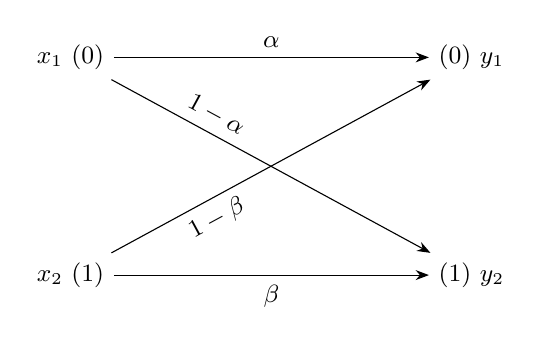
\begin{tikzpicture}[>=Stealth,node distance=2.2cm and 4cm,
   every node/.style={font=\small}]
  \node (x1) {$x_1\ (0)$};
  \node (x2) [below=of x1] {$x_2\ (1)$};
  \node (y1) [right=of x1] {$(0)\ y_1$};
  \node (y2) [below=of y1] {$(1)\ y_2$};
  \draw[->] (x1) -- node[above]{$\alpha$} (y1);
  \draw[->] (x1) -- node[pos=.3,above,sloped]{$1-\alpha$} (y2);
  \draw[->] (x2) -- node[pos=.3,below,sloped]{$1-\beta$} (y1);
  \draw[->] (x2) -- node[below]{$\beta$} (y2);
\end{tikzpicture}
\end{center}

% ---------- Q12 : diagram 6 ----------
\clearpage
\section*{Q12 --- diagram 6}
\begin{center}
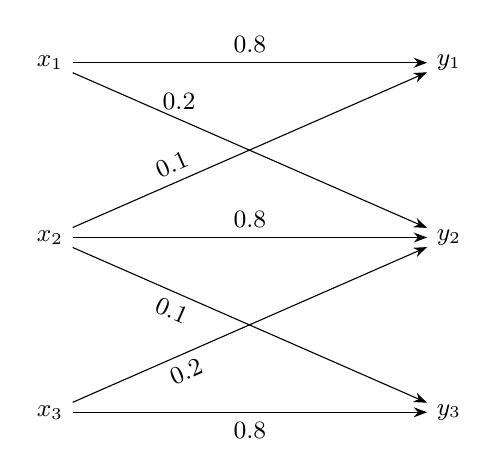
\begin{tikzpicture}[>=Stealth,node distance=1.8cm and 4.5cm,
   every node/.style={font=\small}]
  \node (x1) {$x_1$};
  \node (x2) [below=of x1] {$x_2$};
  \node (x3) [below=of x2] {$x_3$};
  \node (y1) [right=of x1] {$y_1$};
  \node (y2) [right=of x2] {$y_2$};
  \node (y3) [right=of x3] {$y_3$};
  \draw[->] (x1) -- node[above]{$0.8$} (y1);
  \draw[->] (x1) -- node[pos=.3,above]{$0.2$} (y2);
  \draw[->] (x2) -- node[pos=.3,above,sloped]{$0.1$} (y1);
  \draw[->] (x2) -- node[above]{$0.8$} (y2);
  \draw[->] (x2) -- node[pos=.3,below,sloped]{$0.1$} (y3);
  \draw[->] (x3) -- node[pos=.3,below,sloped]{$0.2$} (y2);
  \draw[->] (x3) -- node[below]{$0.8$} (y3);
\end{tikzpicture}
\end{center}

% ---------- Q13 : diagram 7 ----------
\clearpage
\section*{Q13 --- diagram 7}
\begin{center}
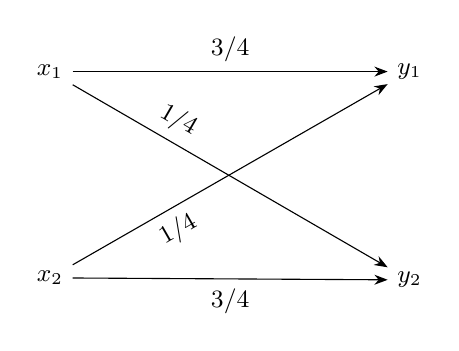
\begin{tikzpicture}[>=Stealth,node distance=2.2cm and 4cm,
   every node/.style={font=\small}]
  \node (x1) {$x_1$};
  \node (x2) [below=of x1] {$x_2$};
  \node (y1) [right=of x1] {$y_1$};
  \node (y2) [below=of y1] {$y_2$};
  \draw[->] (x1) -- node[above]{$3/4$} (y1);
  \draw[->] (x1) -- node[pos=.3,above,sloped]{$1/4$} (y2);
  \draw[->] (x2) -- node[pos=.3,below,sloped]{$1/4$} (y1);
  \draw[->] (x2) -- node[below]{$3/4$} (y2);
\end{tikzpicture}
\end{center}

\end{document}
